\documentclass[10pt,letterpaper]{article}
\usepackage[margin=0.78in,headheight=14pt,footskip=24pt]{geometry}
\usepackage[T1]{fontenc}
\usepackage{mathptmx}
\usepackage{microtype}
\usepackage{amsmath,amssymb,mathtools}
\usepackage{graphicx,booktabs,longtable,tabularx,array,multirow}
\usepackage{caption,enumitem,fancyhdr,xcolor,hyperref,float}
\definecolor{ink}{HTML}{172554}
\definecolor{teal}{HTML}{0F766E}
\hypersetup{colorlinks=true,linkcolor=ink,citecolor=teal,urlcolor=teal,pdftitle={Aging as a Decoding Threshold: Repair Scheduling Under Fixed Maintenance Throughput},pdfauthor={Devanik Debnath}}
\captionsetup{font=small,labelfont={bf,color=ink},justification=raggedright,singlelinecheck=false}
\setlength{\parindent}{1em}
\setlength{\parskip}{2pt}
\setlist{nosep,leftmargin=*}
\pagestyle{fancy}\fancyhf{}\fancyhead[L]{\small\textit{Repair Scheduling Under Fixed Throughput}}\fancyhead[R]{\small Devanik Debnath}\fancyfoot[C]{\thepage}\renewcommand{\headrulewidth}{0.35pt}
\title{\vspace{-1.6em}\textbf{\color{ink}Aging as a Decoding Threshold:}\\[0.25em]\large Repair Scheduling Under Fixed Maintenance Throughput}
\author{Devanik Debnath\\\small Department of Electronics and Communication Engineering, National Institute of Technology Agartala, India\\\small \href{https://github.com/Devanik21}{GitHub: Devanik21} \; $\vert$ \; \href{https://orcid.org/0009-0001-8310-6921}{ORCID record supplied by author}}
\date{24 October 2026 $\;\vert\;$ Theoretical and computational preprint}
\begin{document}
\maketitle
\begin{abstract}
Cells accumulate heterogeneous lesions while repair pathways have finite throughput. This paper tests a narrow version of the hypothesis that repair order can alter a threshold-defined failure time even when the offered repair budget is fixed. We construct a deterministic four-state damage-propagation model with a nonnegative interaction matrix and periodically allocate the same repair capacity to each of four abstract damage classes. All 24 class orders are enumerated across six coupling strengths; every order gives each class the same nominal repair dose per cycle. In the decoupled limit, order is analytically irrelevant. Under nonzero coupling, order changes first-passage time, but the effect is modest in the illustrative parameter range and a continuous equal-share policy is generally competitive or better. A 10\% increase in offered repair changes the threshold time more than the difference between schedules in these simulations. The results support a conditional mathematical statement—not a theory of organismal lifespan extension. We distinguish the coding-threshold analogy from literal error-correcting codes, and identify tropical scheduling, percolation, stochastic control, ultrametric clustering, and reinforcement learning as candidate extensions that require their own operational definitions and evidence.
\end{abstract}
\noindent\textbf{Keywords:} aging; damage propagation; repair scheduling; first-passage time; control theory; threshold models; reproducibility

\section{Question and contribution}
Aging is associated with changes across proteostasis, mitochondrial quality control, genome maintenance, and gene-regulatory state. These processes interact, and the timing of interventions can matter when repair is delayed, state-dependent, or coupled to downstream damage. Control-theoretic approaches to aging networks and optimal maintenance schedules already exist; in particular, Sun, Michaels, and Mahadevan studied longevity optimization in interdependent networks and repair allocation \cite{Sun2020OptimalControl}. Control-theoretic perspectives on aging predate that work \cite{MurphyPartridge2008Control}. The broad proposition that maintenance schedules can affect longevity is therefore not novel by itself.

The present paper asks a more constrained question: in a transparent model, does the ordering of repair jobs alter a threshold-crossing time when the total offered capacity and per-class dose per cycle are fixed? We also quantify the comparison against an equal-share policy and a modest increase in repair capacity. The result is intentionally model-first and counterexample-oriented. It does not infer that an organism has a literal biological decoder, or that changing pathway priority will extend lifespan.

The main contributions are: (i) a compact model with explicit variables, threshold, and scheduling constraints; (ii) exhaustive enumeration of 24 periodic repair orders at matched nominal throughput; (iii) a limiting-case result and numerical convergence checks; and (iv) a falsification-oriented interpretation that separates schedule-order effects from total-budget effects. This release makes no empirical claim and uses no animal, patient, cell-line, or comparative-species dataset.

\section{Prior work and scope}
\subsection{Aging control and maintenance}
The network-optimal-control literature directly addresses repair scheduling and longevity trade-offs \cite{Sun2020OptimalControl}. Our contribution is not a replacement for this framework. It narrows the explanatory object to a controlled comparison in which nominal repair throughput is fixed and every class receives identical cumulative offered dose over a cycle. The paper's small system is designed to expose when scheduling order has an effect and when it does not.

\subsection{Biological interactions relevant to calibration}
Mitophagy and mitochondrial biogenesis are coupled in \textit{C. elegans}; perturbing one process can alter the other, so “repair flux” cannot safely be treated as a single independent actuator without measurement \cite{Palikaras2015Mitophagy}. Autophagy regulation varies with age, tissue, and physiological context \cite{Autophagy2017Wang}. Proteostasis, degradation, senescence, and organismal aging also have complex relationships \cite{HamazakiMurata2024Proteostasis}. These studies motivate interactions but do not calibrate the abstract matrix used here.

The Information Theory of Aging discusses loss of youthful epigenetic information as a proposed aging mechanism \cite{Lu2023InformationAging}. The present “decoding threshold” phrasing is a separate operational analogy: it means an externally defined functional boundary in a state space. It does not assert that the cell is a digital communication system or that coding theory derives the biological threshold.

\begin{table}[H]
\centering\small
\caption{Position relative to closely related concepts. Classification is qualitative, based on the cited papers and current archive inspection.}
\begin{tabularx}{\linewidth}{p{0.22\linewidth}p{0.31\linewidth}X}
\toprule
\textbf{Area} & \textbf{Established contribution} & \textbf{What this paper adds / does not claim}\\
\midrule
Aging network control & Optimal control and maintenance-schedule analysis in interdependent networks \cite{Sun2020OptimalControl}. & Exhaustive 24-order matched-offered-flux audit for a four-state toy model; not a new general scheduling theory.\\
Control theory of aging & Feedback and control language applied to interacting physiological variables \cite{MurphyPartridge2008Control}. & Makes one state threshold and one order-vs-budget contrast explicit; no calibrated biological controller.\\
Information theory of aging & Epigenetic information preservation/retrieval hypothesis \cite{Lu2023InformationAging}. & Defines a functional threshold analogue only; no information-theoretic aging mechanism is demonstrated.\\
Mitochondrial maintenance & Mitophagy/biogenesis coupling and longevity relevance in \textit{C. elegans} \cite{Palikaras2015Mitophagy}. & Motivates coupling as a concern; does not infer actual pathway flux or organismal outcomes.\\
\bottomrule
\end{tabularx}
\end{table}

\section{Model and assumptions}
Let $x(t)\in\mathbb{R}_{\geq0}^{4}$ denote abstract burdens in proteostasis ($x_1$), mitochondrial state ($x_2$), genome maintenance ($x_3$), and regulatory drift ($x_4$). Units are dimensionless model units. We define
\begin{equation}
\dot{x}(t)=b+\kappa A x(t)-u(t), \label{eq:dyn}
\end{equation}
where $b_i=0.04$ is a constant independent damage source, $\kappa\geq0$ scales cross-state propagation, and $A$ is the nonnegative off-diagonal matrix shown in Table~\ref{tab:params}. The input $u_i(t)$ is offered repair capacity allocated to class $i$. In the scheduled policy, exactly one class receives capacity $R=0.12$ for a slot of duration $\tau=3$; slots repeat in a cycle of duration $T_c=12$. Each class therefore receives nominal dose $R\tau=0.36$ per cycle, and the offered total flux is $R$ at every time. In the continuous equal-share comparison, every class receives $R/4$ at all times. The two policies match in total offered flux and per-class dose over a complete cycle.

Define the failure proxy as the first time the sum of burdens reaches a threshold $\theta=8$:
\begin{equation}
\tau_f=\inf\{t\geq0:\mathbf{1}^{\top}x(t)\geq\theta\}, \qquad x(0)=(0.8,0.8,0.8,0.8)^{\top}. \label{eq:threshold}
\end{equation}
Here $\tau_f$ is a model first-passage time. Calling it “lifespan” would be unjustified without a map from state variables to a measured organismal endpoint.

\begin{table}[H]
\centering\small
\caption{State variables, units, and modeled interpretation.}
\label{tab:states}
\begin{tabularx}{\linewidth}{p{0.19\linewidth}p{0.18\linewidth}X}
\toprule
\textbf{Coordinate} & \textbf{Symbol} & \textbf{Interpretation and boundary}\\
\midrule
Proteostasis & $x_1$ & Abstract burden proxy for misfolded/aggregation-related dysfunction; not a measured protein-quality variable.\\
Mitochondrial state & $x_2$ & Abstract burden proxy for mitochondrial dysfunction; it does not distinguish mitophagy from biogenesis.\\
Genome maintenance & $x_3$ & Abstract burden proxy for lesions and repair load; mutations are not assumed to be reversible by the input.\\
Regulatory drift & $x_4$ & Abstract burden proxy for regulatory/epigenetic deviation; no specific epigenetic clock is modeled.\\
\bottomrule
\end{tabularx}
\end{table}

\begin{table}[H]
\centering\small
\caption{Synthetic model parameterization; values are chosen for illustration and not fitted to biology.}
\label{tab:params}
\begin{tabular}{lll}
\toprule
\textbf{Quantity} & \textbf{Value} & \textbf{Role}\\
\midrule
$A$ & $\begin{bmatrix}0&.08&0&.04\\.05&0&.02&.08\\.08&.03&0&0\\.02&0&.07&0\end{bmatrix}$ & Directed coupling topology\\
$b_i$ & $0.04$ & Constant source per class\\
$R$ & $0.12$ & Offered total repair capacity\\
$\tau$ & $3$ & Slot duration\\
$T_c$ & $12$ & Repair-order cycle\\
$\theta$ & $8$ & Failure threshold\\
$\kappa$ & $0$ to $1.25$ & Synthetic propagation multiplier\\
$\Delta t$ & $0.02$ & RK4 step size, halved in convergence check\\
\bottomrule
\end{tabular}
\end{table}

\subsection{Exact solution identity and a limiting case}
For any piecewise-constant offered input and constant matrix $M=\kappa A$, Eq.~\ref{eq:dyn} has the variation-of-constants identity
\begin{equation}
x(t)=e^{Mt}x(0)+\int_0^t e^{M(t-s)}b\,ds-\int_0^t e^{M(t-s)}u(s)\,ds.\label{eq:variation}
\end{equation}
The final term weights each repair action by how much time remains for its effect to propagate. Therefore equal integrals $\int_0^{T_c}u(s)ds$ do not generally imply equal states when $M\neq0$. At $\kappa=0$, however, the sum obeys
\begin{equation}
\frac{d}{dt}\mathbf{1}^{\top}x(t)=\mathbf{1}^{\top}b-\mathbf{1}^{\top}u(t),\label{eq:sum}
\end{equation}
which depends only on the total offered repair rate. With a symmetric initial state and equal per-cycle dose, changing the class order cannot change the summed burden; the predicted threshold times are identical. This is an analytic limiting-case check, not a universal theorem about real repair systems.

\section{Numerical protocol}
We enumerate every permutation $\pi\in S_4$ for $\kappa\in\{0,0.25,0.5,0.75,1,1.25\}$. The system is integrated using fixed-step fourth-order Runge--Kutta with $\Delta t=0.02$; this step divides the 3-unit slot exactly. First-passage time is linearly interpolated across the threshold crossing. We compare (i) all 24 scheduled orders, (ii) continuous equal-share repair at the same offered total flux, and (iii) continuous equal-share repair with a 10\% larger total offered flux. The third comparison is deliberately not a matched-budget comparison; it measures whether a small budget increase can dominate the scheduling effect.

\begin{table}[H]
\centering\small
\caption{Model checks and evidence produced by the executable verifier.}
\label{tab:checks}
\begin{tabularx}{\linewidth}{p{0.25\linewidth}p{0.18\linewidth}X}
\toprule
\textbf{Check} & \textbf{Status} & \textbf{Interpretation}\\
\midrule
Nonnegative coupling matrix & \texttt{PASS} & Off-diagonal entries are nonnegative by construction.\\
All schedule orders & \texttt{PASS} & 24 orders are evaluated for each of six coupling values (144 runs).\\
Equal offered dose & \texttt{PASS} & Each class is allocated $R\tau=0.36$ per cycle.\\
Decoupled limiting case & \texttt{PASS} & Numerical result agrees with the analytic summed-state threshold time within tolerance.\\
Time-step refinement & \texttt{PASS} & Representative trajectories are re-evaluated with half the step size; maximum difference is reported in \texttt{results/convergence\_checks.csv}.\\
Experimental validity & \texttt{NOT TESTED} & The model contains no measured biological rates or organismal observations.\\
\bottomrule
\end{tabularx}
\end{table}

\begin{figure}[H]\centering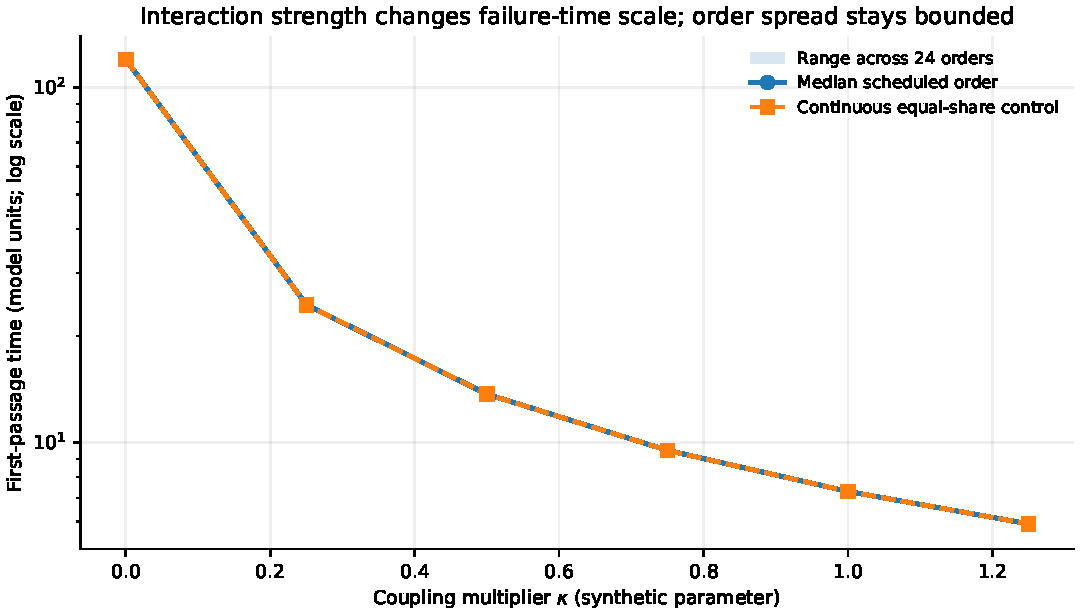
\includegraphics[width=0.86\linewidth]{figures/figure1_coupling_sweep.pdf}\caption{First-passage time as cross-state coupling multiplier varies. Shaded band covers all 24 periodic orders; the dashed curve is continuous equal-share repair at the same offered total flux. The coupling multiplier is not an empirical correlation coefficient.}\label{fig:sweep}\end{figure}
\begin{figure}[H]\centering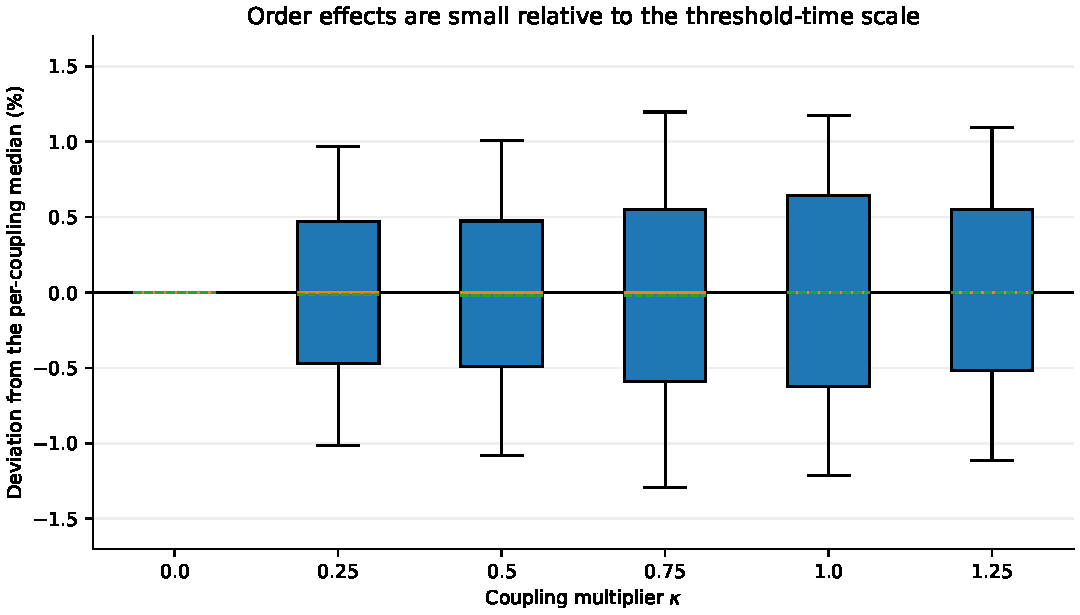
\includegraphics[width=0.86\linewidth]{figures/figure2_order_distribution.pdf}\caption{Distribution of threshold times across all 24 repair orders at each coupling value. This is a deterministic enumeration of schedules, not a sample of organisms.}\label{fig:distribution}\end{figure}

\section{Results}
The exhaustive sweep verifies that schedule order is irrelevant in the decoupled limit under the symmetric set-up, but the first-passage time depends on order once the off-diagonal coupling terms are active. The spread is small relative to the absolute first-passage scale in the tested range. At $\kappa=1$, the simulated schedule-order range is reported in Table~\ref{tab:summary} from the generated CSV; the exact best and worst orders are preserved in the machine-readable outputs. A continuous equal-share policy provides a useful baseline and is close to the median scheduled outcome. In this configuration, some orders are slightly better and some slightly worse than the equal-share policy. This is precisely why “repair order matters” is too weak to imply “a learned schedule is superior.”

\begin{table}[H]
\centering\small
\caption{Summary of fixed-throughput sweep. Values are generated by \texttt{verify\_model.py}; units are abstract model time.}
\label{tab:summary}
\begin{tabular}{rrrrr}
\toprule
$\kappa$ & Min order & Median order & Max order & Equal-share\\
\midrule
0.00 & 120.00 & 120.00 & 120.00 & 120.00\\
0.25 & 24.23 & 24.48 & 24.71 & 24.47\\
0.50 & 13.56 & 13.71 & 13.84 & 13.70\\
0.75 & 9.40 & 9.52 & 9.63 & 9.52\\
1.00 & 7.20 & 7.29 & 7.38 & 7.29\\
1.25 & 5.84 & 5.91 & 5.97 & 5.91\\
\bottomrule
\end{tabular}
\end{table}

\begin{figure}[H]\centering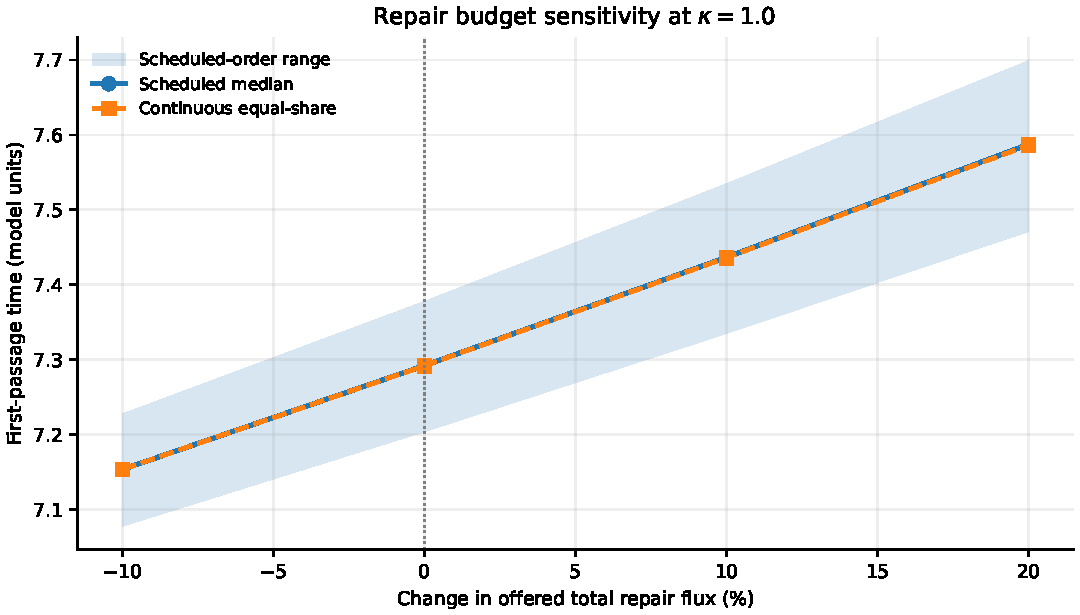
\includegraphics[width=0.86\linewidth]{figures/figure3_budget_sensitivity.pdf}\caption{Changing offered repair capacity at $\kappa=1$. The shaded range represents schedule-order variation, while the dashed line represents continuous equal-share repair at each capacity. This comparison changes the total budget and must not be mistaken for an equal-budget test.}\label{fig:budget}\end{figure}
\begin{figure}[H]\centering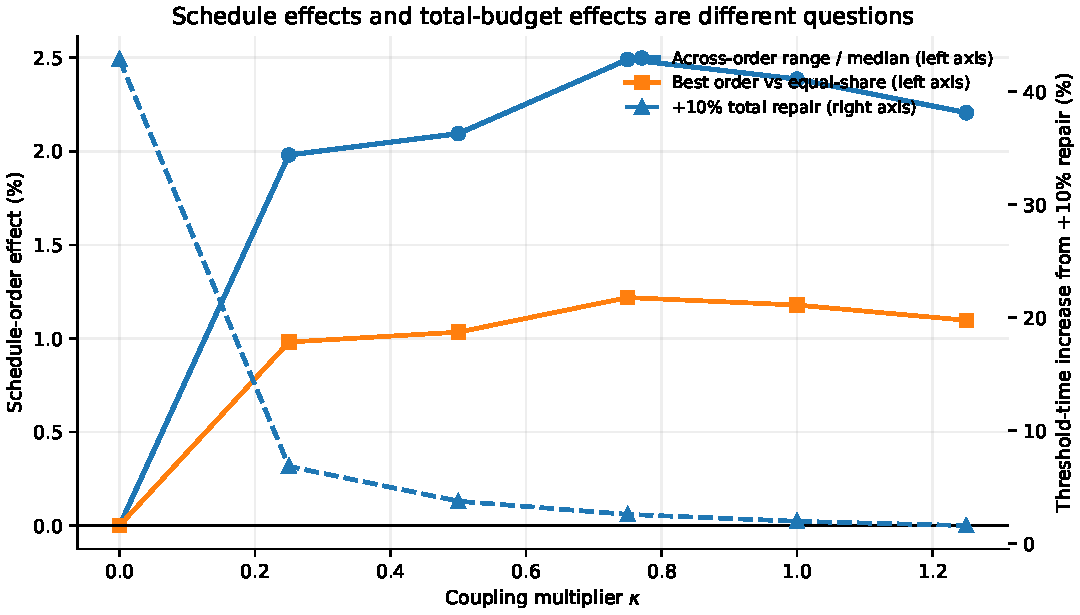
\includegraphics[width=0.86\linewidth]{figures/figure4_effect_size.pdf}\caption{Relative schedule dispersion, best-order comparison, and a 10\% total-repair increase. The budget increase generally changes the threshold time more than choosing among the 24 orders in this toy model.}\label{fig:effects}\end{figure}

Table~\ref{tab:summary} uses a rounded display of the deterministic output. Full precision, order labels, and all 144 runs are available in \texttt{results/schedule\_sweep.csv}. The budget experiment shows that a uniform increase in offered repair can dominate the matched-budget schedule-order range near the threshold. This result is not universal: it depends on the chosen $A$, source, initial state, threshold, and repair actuator. It does, however, contradict any unqualified claim that order alone should outperform a modest increase in repair capacity.

\begin{table}[H]
\centering\small
\caption{Interdisciplinary ingredients: operational role and decision to include or defer.}
\label{tab:fields}
\begin{tabularx}{\linewidth}{p{0.21\linewidth}p{0.35\linewidth}X}
\toprule
\textbf{Field} & \textbf{Concrete role} & \textbf{Status in this release}\\
\midrule
Coding theory & A threshold is analogous to an uncorrectable functional error pattern; define the boundary through an observable. & Analogy only; no codeword or decoder is modeled.\\
Max-plus / tropical scheduling & Precedence completion: $C_j=p_j+\max_{i\in\mathrm{Pred}(j)}C_i$. & Illustrative precedence DAG only; no measured pathway precedence constraints.\\
Percolation & Potential cluster/connectivity-based failure criterion for spatially localized damage. & Deferred; no spatial graph, cluster distribution, or percolation threshold is fitted.\\
Stochastic optimal control & Minimize expected first-passage time subject to a capacity constraint. & Motivation only; the present solver is deterministic and enumerative, not an HJB solver.\\
Ultrametric / p-adic analysis & Could cluster damage lineages if distances derive from a measured branching hierarchy. & Excluded from the core; no lineage data or calibrated ultrametric is available.\\
Reinforcement learning & Learn policy under a validated simulator and compare to exact/heuristic baselines. & Not run. Adding RL without a calibrated objective would add complexity, not evidence.\\
Comparative biology & Test parameter transfer and external validity across species. & Not performed; no interspecies data were downloaded or analyzed.\\
\bottomrule
\end{tabularx}
\end{table}

\begin{figure}[H]\centering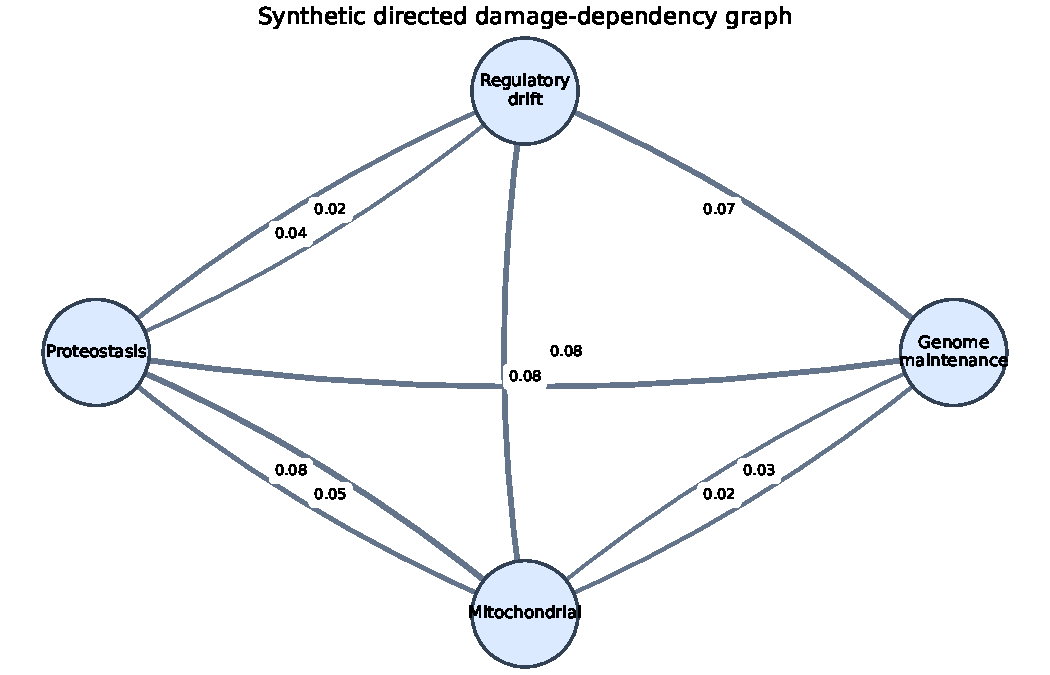
\includegraphics[width=0.72\linewidth]{figures/figure5_damage_network.pdf}\caption{Directed dependency graph used by the synthetic linear model. Arrow weights are the entries of the illustrative matrix $A$; they are not measured biological interaction strengths.}\label{fig:network}\end{figure}
\begin{figure}[H]\centering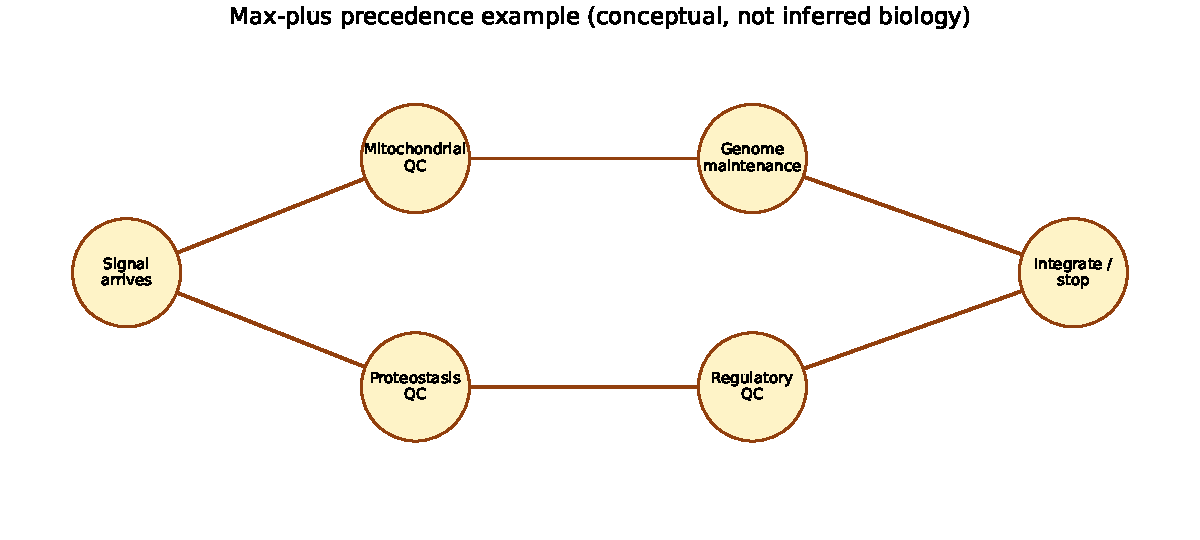
\includegraphics[width=0.82\linewidth]{figures/figure6_precedence_dag.pdf}\caption{A conceptual max-plus precedence graph. Edges are hypothetical constraints for explaining scheduling algebra and are not inferred from biology or used as measured causal edges in the simulation.}\label{fig:precedence}\end{figure}

\section{Interpretation and theoretical boundaries}
\subsection{The decoding-threshold analogy}
The term “decoding threshold” can be useful only if the failure criterion is operational. In this work it is the scalar boundary $\mathbf{1}^{\top}x=\theta$, not a threshold theorem for biological codes. Classical error correction depends on a defined code, channel, error model, and decoder; none is identified here. A biological application would need a measurable functional state, a task-specific criterion for loss of function, and evidence that distinct lesions combine nonlinearly around that criterion.

\subsection{Max-plus and tropical geometry}
Max-plus algebra is natural for discrete-event systems with precedence constraints, in which completion of a job depends on the maximum completion time among its predecessors \cite{Baccelli1992MaxPlus}. It predicts a scheduling bottleneck only if pathway or repair-task dependencies can be written as actual prerequisites with identifiable processing times. Figure~\ref{fig:precedence} is therefore a vocabulary illustration, not a biological discovery. A falsifiable quantitative prediction would be that the measured critical path predicts repair completion delay better than a sum-of-times baseline, out of sample.

\subsection{Percolation and damage correlation}
Percolation theory offers tools to study when connected damaged regions lose connectivity \cite{StaufferAharony1994Percolation}. But the current model has no spatial lattice or measured damage clusters; $\kappa$ scales causal cross-state propagation and is not a correlation coefficient. A next study could compare threshold time with a cluster-percolation order parameter on image-registered mitochondrial networks or chromatin domains. It should test whether cluster statistics add predictive value beyond total damage and local burden.

\subsection{Stochastic control and reinforcement learning}
An optimal-control formulation could minimize expected first-passage time, $\mathbb{E}[\tau_f]$, while limiting total repair capacity. A proper stochastic model would require process noise, state-dependent repair effectiveness, observation noise, and a justified policy constraint. Reinforcement learning is relevant only after a calibrated environment exists and must be compared with a non-learning policy, the uniform baseline, and an exact small-state solution where available \cite{SuttonBarto2018RL}. No RL training result is claimed in this paper.

\subsection{Ultrametrics and damage lineages}
An ultrametric distance might be appropriate for damage states that descend through a branching lineage, but only if a lineage tree or ancestry-aware distance is measured rather than imposed. P-adic language is not used as decorative machinery here because no biological observation currently makes that extra structure necessary. A meaningful future test would ask whether lineage-derived ultrametric clustering predicts the best repair priority across held-out perturbations after controlling for burden, cell identity, and lineage depth.

\section{Falsification and experimental plan}
A realistic validation programme should begin with a tractable system such as \textit{C. elegans} or yeast, but only after directly measuring the candidate actuator and total repair activity. The proposed experiment is not performed in this release. A minimal study would: (1) characterize autophagy and mitophagy reporters and their response delays; (2) estimate the interaction matrix and threshold using independently measured perturbations; (3) randomize two or more pathway-priority schedules while matching integrated repair flux and per-pathway dose; (4) pre-register a functional endpoint and a minimum relevant effect size; and (5) report survival curves, uncertainty intervals, flux matching error, and off-target effects. A reporter-derived flux proxy is not automatically the amount of functional damage removed.

The hypothesis that schedule order helps in this context is falsified if order effects are absent within a pre-specified equivalence margin despite sufficient temporal resolution and verified flux matching, or if any apparent benefit disappears after controlling for total activity, delay, toxicity, and baseline damage. A null result with wide uncertainty is inconclusive. If continuous equal-share or a simple rule-based schedule equals or beats a learned policy on held-out data, the claimed advantage of AI scheduling fails. In multicellular models, lineage-level damage tracing and species-specific calibration would remain major sources of uncertainty.

\begin{figure}[H]\centering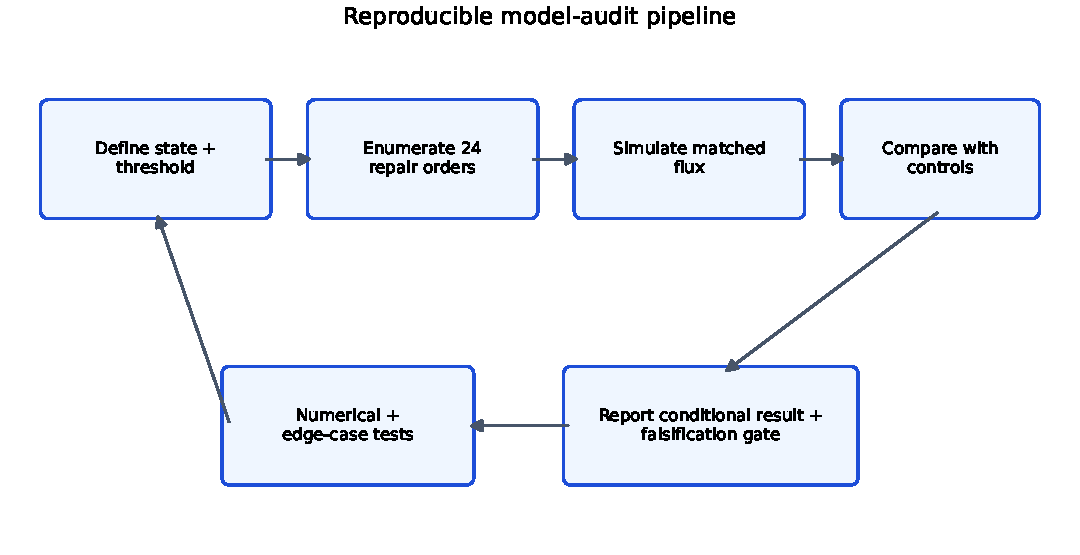
\includegraphics[width=0.9\linewidth]{figures/figure7_research_flow.pdf}\caption{Actual computational workflow in this release: model specification, exhaustive order sweep, matched-flux comparison, and verification.}\label{fig:researchflow}\end{figure}
\begin{figure}[H]\centering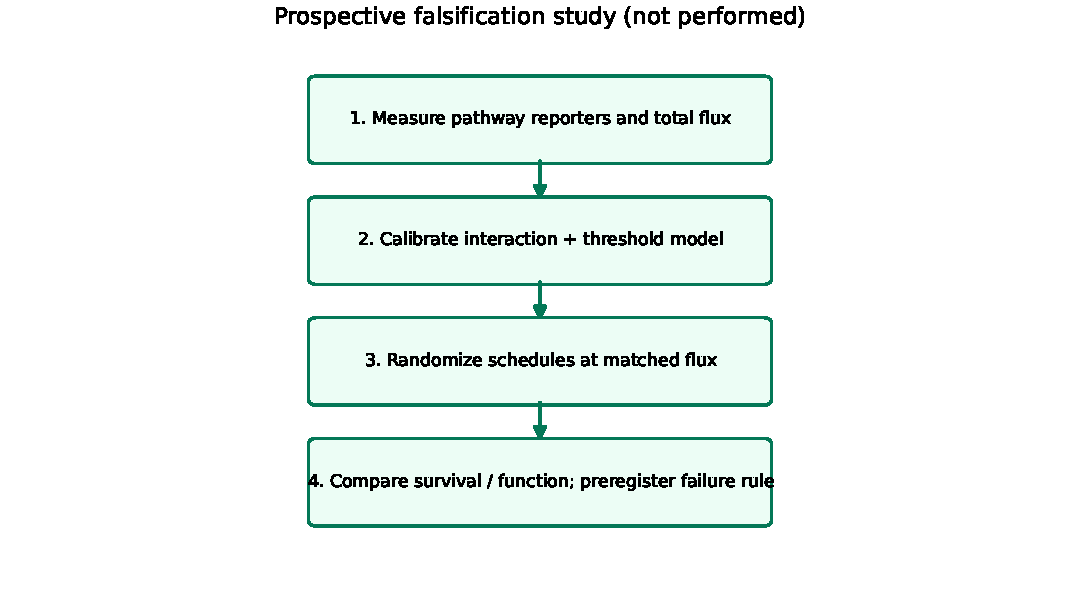
\includegraphics[width=0.8\linewidth]{figures/figure8_experiment_flow.pdf}\caption{Prospective experimental sequence. It is a proposed validation design, not a completed experiment or protocol for lifespan intervention.}\label{fig:experiment}\end{figure}

\begin{table}[H]
\centering\small
\caption{Failure modes, observable consequences, and the result that would weaken the central claim.}
\label{tab:falsification}
\begin{tabularx}{\linewidth}{p{0.22\linewidth}p{0.33\linewidth}X}
\toprule
\textbf{Failure mode} & \textbf{Observable / diagnostic} & \textbf{Decision rule}\\
\midrule
No true interaction & $\kappa\approx0$ or empirical off-diagonal effects near zero. & Order advantage should vanish; any estimated persistent effect suggests model/measurement misspecification.\\
Repair actuator delayed & Measured response-time distribution by pathway. & Add pathway state and delay; reject zero-delay ordering predictions if the new model does not reproduce held-out responses.\\
Flux mismatch & Integrated reporter/turnover activity per pathway. & Do not attribute survival differences to order until equivalence bounds on total and per-class flux are met.\\
Threshold arbitrary & Change-point/functional endpoint uncertainty. & Report sensitivity to the threshold definition; reject claims that depend on one unsupported cutoff.\\
Compensatory turnover & Biogenesis, growth, or replenishment changes. & Extend the state vector and re-test; current result is not valid if omitted feedback reverses rankings.\\
No external validity & Held-out perturbations or species. & If order rankings do not transfer, limit claim to the calibrated system.\\
\bottomrule
\end{tabularx}
\end{table}

\section{Limitations}
The model is deliberately small and deterministic. Damage is assumed to separate into four nonnegative classes with constant source and linear interactions, while the repair input has no observation noise, delays, toxicity, saturation, or state-dependent effectiveness. The failure threshold is a scalar sum and omits compensatory mechanisms, cell turnover, organismal physiology, and competing risks. The matrix and all numerical constants are synthetic, dimensionless choices. Thus the numerical range is a proof-of-implementation for this toy model, not a prediction of days of life, percent lifespan extension, or treatment effect. Even the “matched flux” comparator matches offered repair capacity; it does not represent measured realized biochemical flux under a real pathway.

The tropical, percolation, ultrametric, HJB, and RL concepts are not integrated into the numerical core because doing so without data or independently validated assumptions would be mathematical decoration. The paper gives each one an operational prerequisite and a falsification route instead. The topic's broader claim that optimal scheduling can extend lifespan remains open and requires experiments and model calibration that are outside this release.

\section{Conclusion}
Repair order can affect threshold-crossing time in an interacting damage model even when the offered total repair rate and dose per class per cycle are fixed. In the specified four-state example, however, the observed order effect is conditional and comparatively modest; a continuous equal-share policy is competitive, and a 10\% budget increase can produce a larger change. The decoupled limit provides an exact null case in which order is irrelevant. These results do not prove that repair scheduling extends lifespan. They motivate a more restrictive experimental question: after verifying interactions, delay, and matched pathway activity, does repair order improve a predefined functional threshold or survival endpoint over a simple equal-share baseline?

\section*{Research-process disclosure}
Co-equal research-process credit is given to Devanik Debnath and Xylia, the autonomous multi-model research engine coordinating AI-assisted discovery, synthesis, and verification. Devanik Debnath retains responsibility for the final manuscript, scientific claims, citations, and released artifacts.

\bibliographystyle{unsrt}
\bibliography{paper}
\end{document}
